\documentclass[catalan, a4paper, nobib]{tufte-handout}

% encoding
\usepackage[utf8]{inputenc}
\usepackage[T1]{fontenc}
\usepackage{lmodern}
\usepackage{babel}

\frenchspacing
\usepackage[style=spanish]{csquotes}
\MakeAutoQuote{«}{»}

\usepackage{booktabs}
\usepackage{circuitikz}
\usepackage{siunitx}
\usepackage{amsmath}
\usepackage{nicefrac}
\usepackage{amssymb}

\graphicspath{
    {fotos/}
}

% hyperlink setup / metadata
\usepackage{hyperref}
\AfterPreamble{\hypersetup{
  %%pdfauthor={},
  %%pdftitle={},
  %%pdfsubject={},
}}

% document metadata
\author{Víctor Méndez}
\title{ICOM: Pràctica 5}
\date{22-5-2024}

\begin{document}

\maketitle

\newthought{Activitat 5.1}

Veure la figura \ref{fig:1}. Amb la funció "find peaks" situem dos markers, un al lòbul principal i un a un lòbul secundari. Les mesures extretes son $P_1=\qty[qualifier-mode=combine]{3.3}{\deci\bel\of{m}}$ i $P_2=\qty[qualifier-mode=combine]{-10.43}{\deci\bel\of{m}}$. La relació correspon a $\alpha=P_1-P_2=\qty{10.74}{\deci\bel}$. S'apropa a la relació teòrica.

\begin{figure}
    \begin{center}
        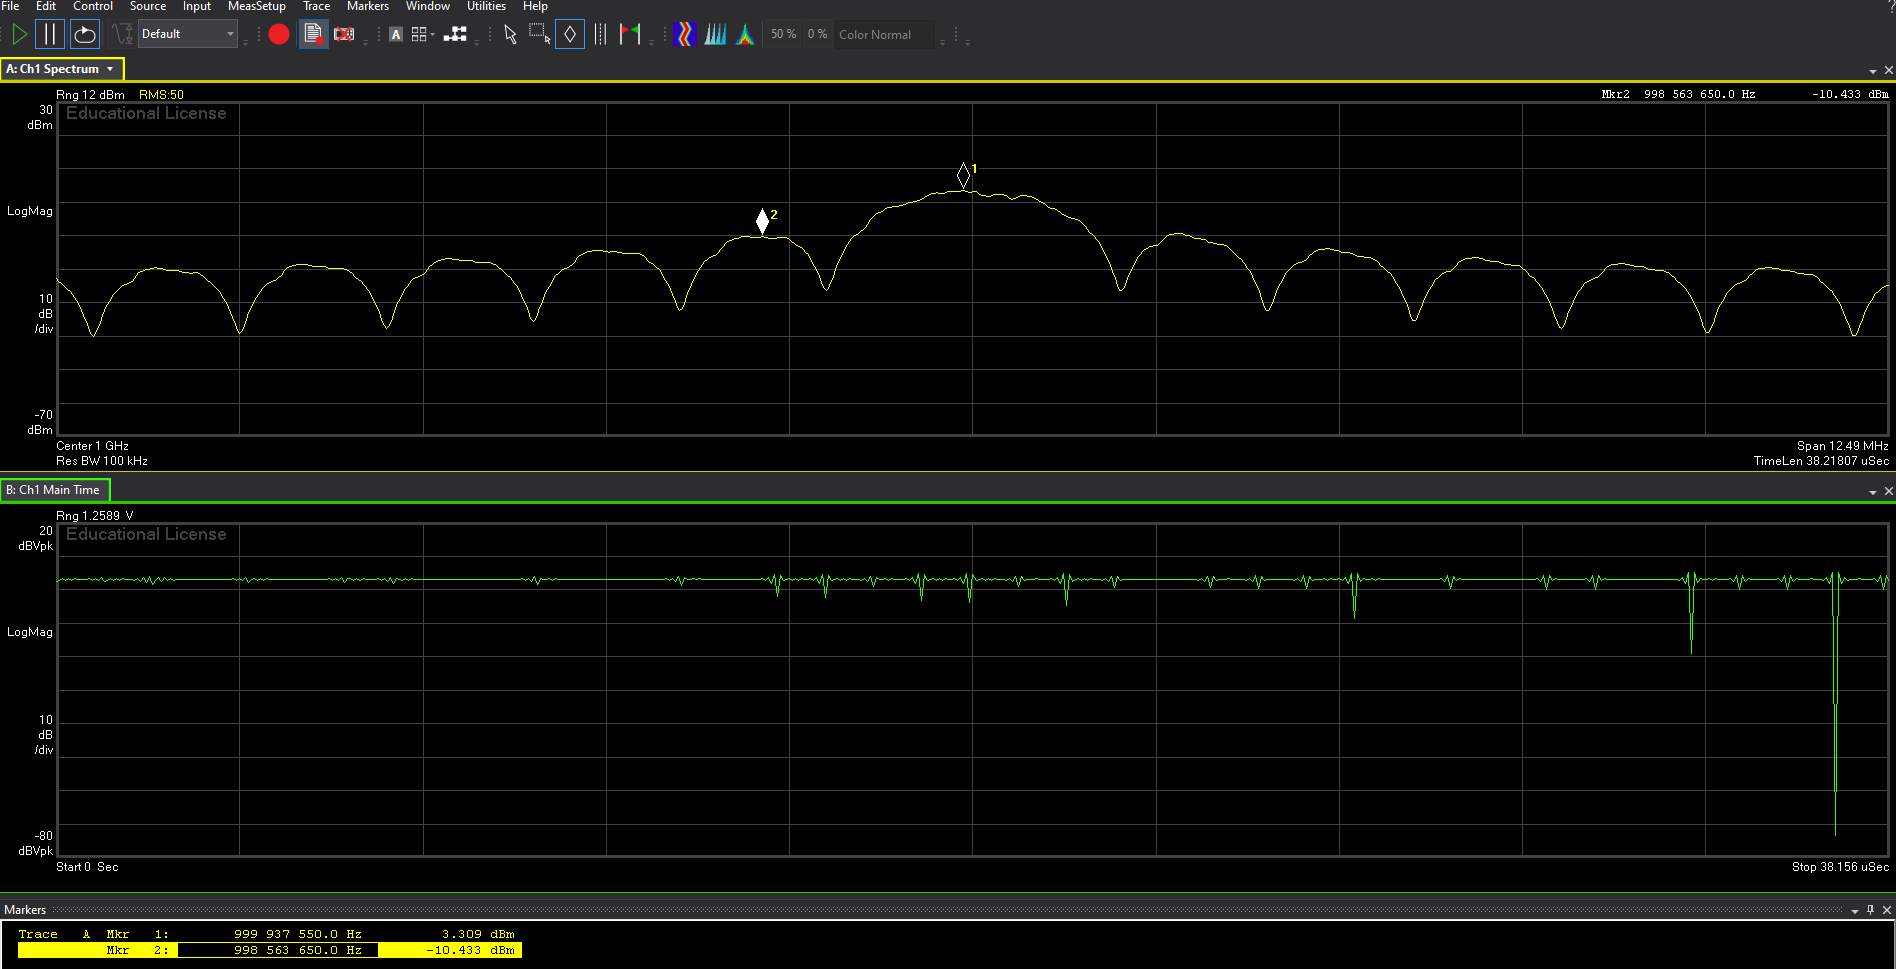
\includegraphics[width=295px]{1.png}
    \end{center}
    \caption{Espectre del senyal QPSK amb \num{50} mostres de mitjana}
    \label{fig:1}
\end{figure}

Com el pols conformador emprat és un pols rectangular de longitud $T$, l'espectre que veiem és una $sinc$ amb una amplada de lòbul principal $\nicefrac{2}{T}$, la seva transformada. Com $r=\nicefrac{1}{T}$ mesurem l'amplada i dividim per \num{2}, $r = \frac{\Delta}{2} \simeq \qty{1}{\mega\hertz}$. Es correspon.\sidenote{El bit-rate $r_b$ emprat al LaVICAD era de \qty{2}{\mega\hertz}. Per tant el symbol-rate val $r=\frac{r_b}{b}=\qty{1}{\mega\hertz}$.}

\newthought{Activitat 5.2}

Veure la figura \ref{fig:2}. Les transicions entre símbols ara son línies rectes. Aquest efecte es degut a que la autocorrelació d'un pols rectangular és un pols triangular.

\begin{figure}
    \begin{center}
        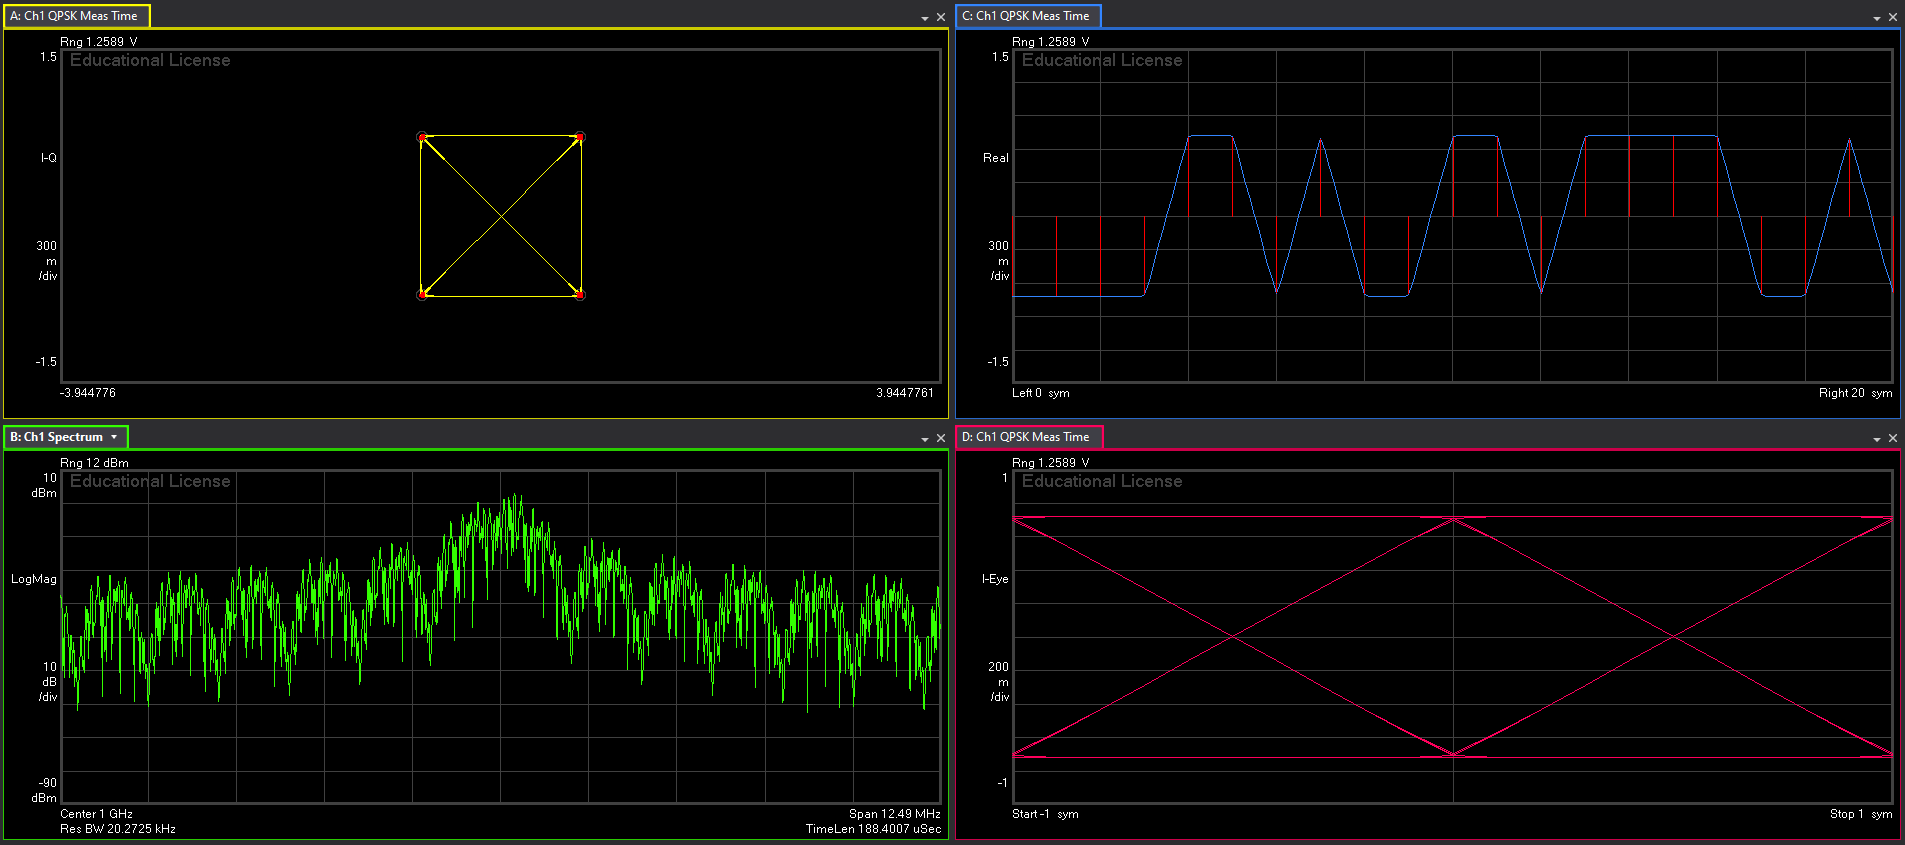
\includegraphics[width=295px]{2.png}
    \end{center}
    \caption{Demodulació d'una QPSK amb pols rectangular com a pols conformador}
    \label{fig:2}
\end{figure}

\newthought{Activitat 5.3}

Veure la figura \ref{fig:3}. La relació entre lobul principal i secundari ha empitjorat. Ara $\alpha = \qty[qualifier-mode=combine]{11}{\deci\bel\of{m}}$.

\begin{figure}
    \begin{center}
        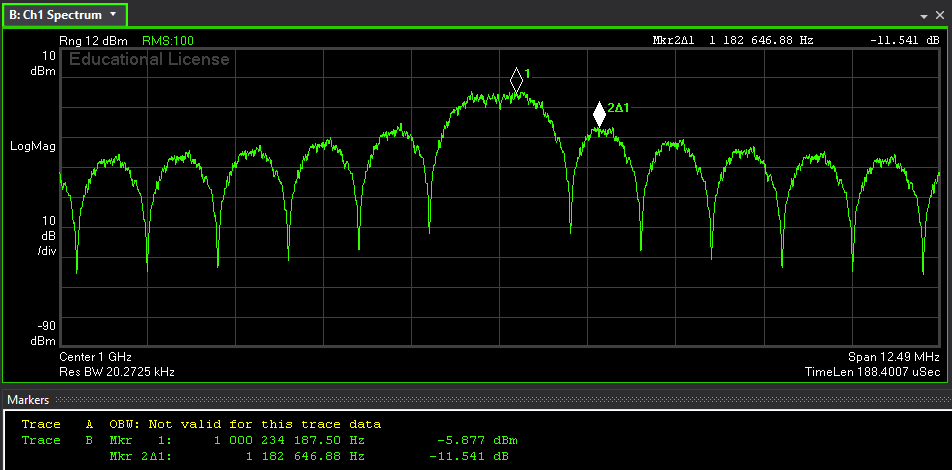
\includegraphics[width=295px]{3.png}
    \end{center}
    \caption{Espectre d'un senyal QPSK amb un canal no ideal}
    \label{fig:3}
\end{figure}

\newthought{Activitat 5.4}

Veure la figura \ref{fig:4}. Un canal no ideal suposa ISI. Com el canal ja no és una Delta sinò dues, cada punt de la cuadratura rebuda s'ha desdoblat en \num{4}. Els efectes es noten a l'espectre (vist a l'apartat anterior), la cuadratura i el diagrama d'ull. En aquest últim s'observa una apertura més petita que \num{1}.

\begin{figure*}
    \begin{center}
        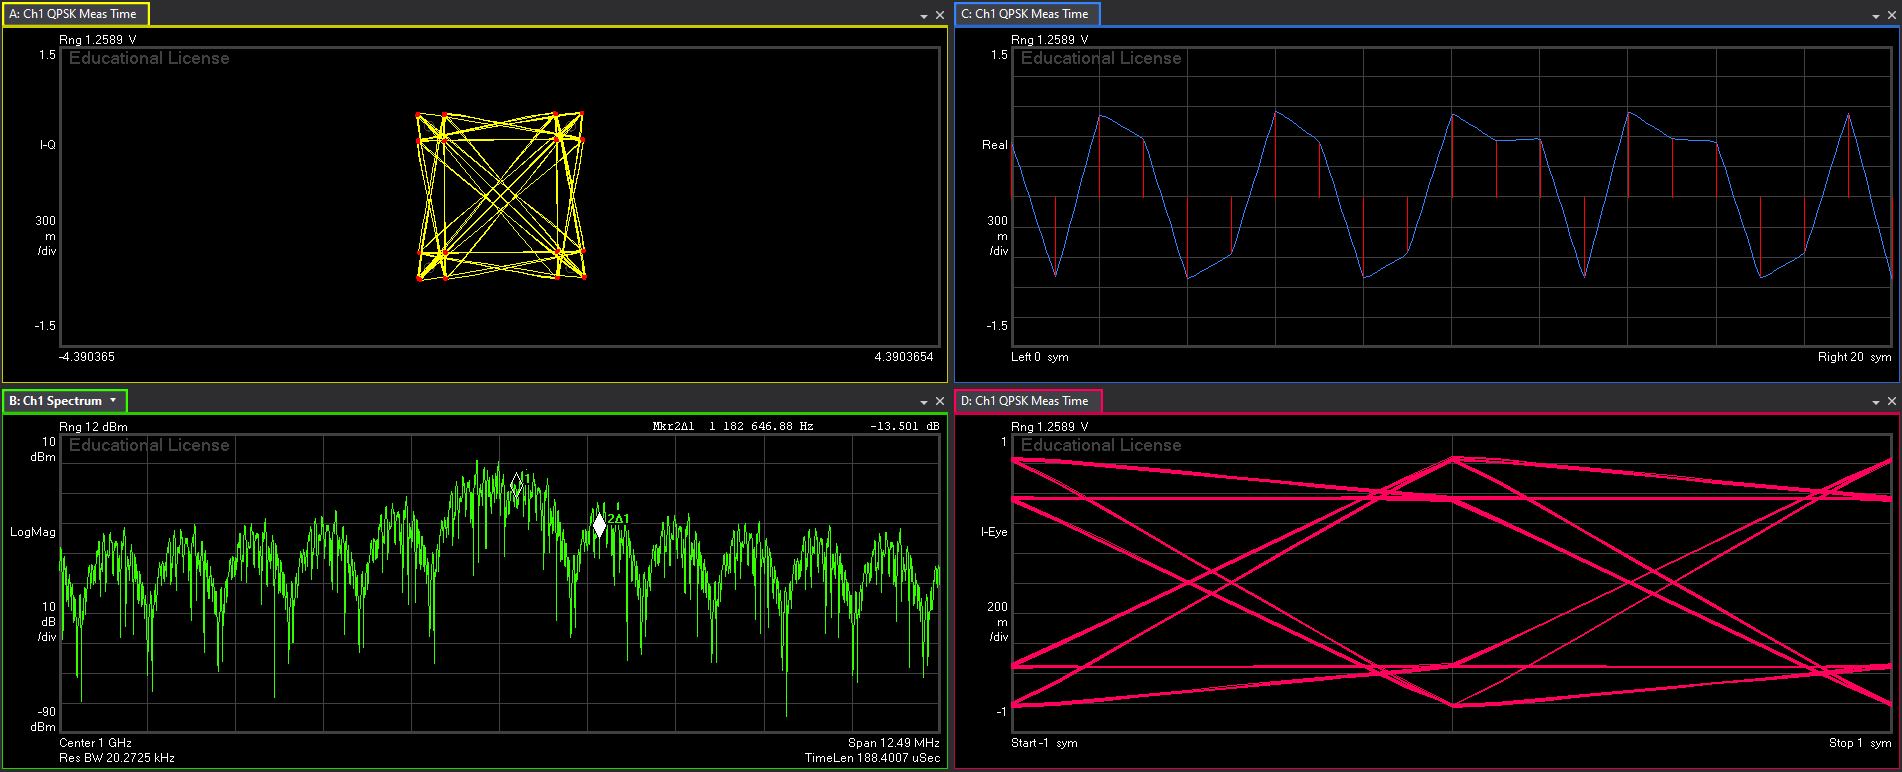
\includegraphics[width=450px]{4.png}
    \end{center}
    \caption{Demodulació d'un senyal QPSK amb un canal no ideal}
    \label{fig:4}
\end{figure*}

\newpage

\newthought{Activitat 5.5}

Veure la figura \ref{fig:5}. La cuadratura ara és un nuvol de punts. Les transicions entre símbols han deixat de ser línies perfectes i ha empitjorat la apertura del diagrama d'ull.

\begin{figure*}
    \begin{center}
        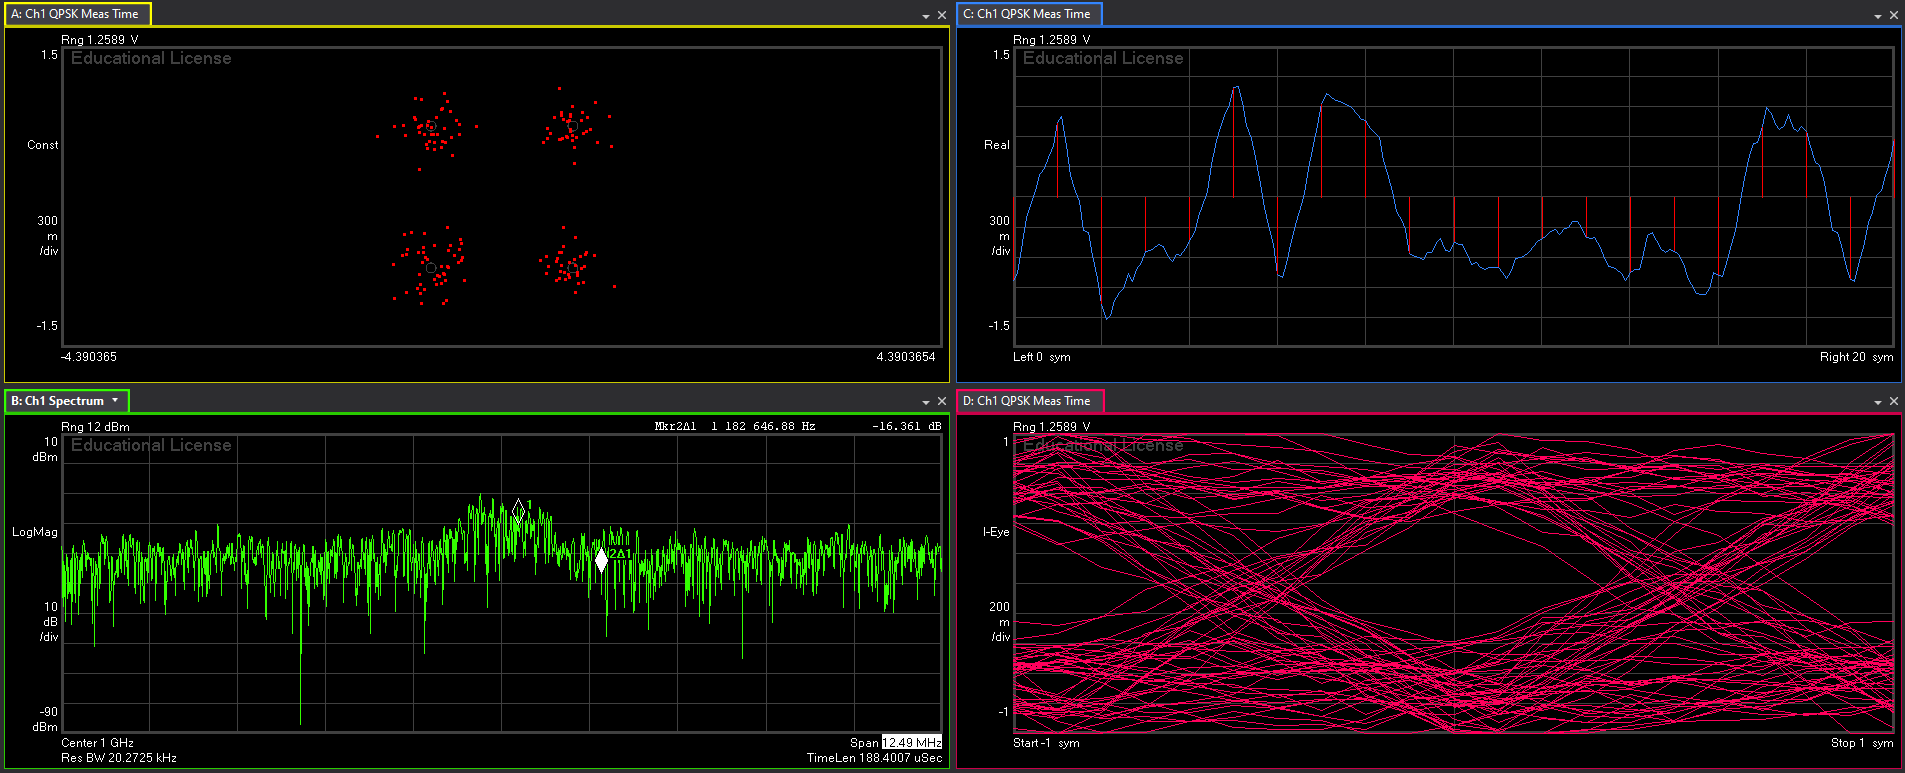
\includegraphics[width=450px]{5.png}
    \end{center}
    \caption{Demodulació d'un senyal QPSK amb soroll i un canal no ideal}
    \label{fig:5}
\end{figure*}

\end{document}